\todo[inline, color=pink, size=normalsize]{Definição sucinta do controle ótimo comparando com o controle clássico e apresentando um exemplo (trajetória a ser percorrida por uma aeronave)}

A Teoria de Controle Clássico pode ser resumidamente descrita como um conjunto de métodos que viabiliza o projeto de controladores que possibilitam a computação da entrada à qual um dado processo deve ser submetido de forma que a saída associada ao mesmo evolua da maneira desejada \cite{franklin_sistemas_2013}. O projeto de um controlador em malha fechada, como são chamados os controladores baseados na realimentação da saída, é realizado por meio de um procedimento iterativo no qual os ganhos associados a uma dada lei de controle, conforme pode ser observado na Figura \ref{fig:introducao:controleMF}. Assim, os controladores são ajustados enquanto o desempenho do processo é verificado a partir de critérios definidos no domínio do tempo, como o máximo sobressinal, o tempo de acomodação, e o tempo de sumida, ou no domínio da frequência, como a margem de fase, a margem de ganho, e a largura de banda \cite{kirk_optimal_2004}. 

\noindent	
\begin{minipage}{\textwidth}
	\vspace{\onelineskip}
	\centering
	\includegraphics[width=1\linewidth]{diag/introducao/pdf/controleMF}
	\captionof{figure}[Sistema de controle em malha fechada]{Sistema de controle em malha fechada.}
	\label{fig:introducao:controleMF}
	\vspace{\onelineskip}
\end{minipage}

No entanto, outros critérios devem ser considerados no controle de sistemas de dinâmica complexa (possuem múltiplas entradas e saídas e que estejam sujeitos a limitações operacionais). Por exemplo, considerando-se a determinação das forças $ F(t) $ a serem impostas sob uma aeronave para que um dado ponto de chegada seja atingido, de forma que sejam evitadas zonas proibitivas, ao mesmo tempo em que minimiza-se o gasto de combustível da aeronave, conforme observado na Figura \ref{fig:introducao:aeronaveControleOtimo}. Vale ressaltar que, nesse caso, os perfis de aceleração $ a(t) $, de velocidade $ v(t) $, e de posição $ P\big(x(t), y(t)\big) $ da aeronave devem ser também determinados. O Controle Ótimo (CO) é uma das ferramentas que possibilita a resolução de problemas desse tipo. 

\noindent	
\begin{minipage}{\textwidth}
	\vspace{\onelineskip}
	\centering
	\includegraphics[width=0.7\linewidth]{draw/introducao/pdf/aviaoControleOtimo}
	\captionof{figure}[Trajetória ótima a ser percorrida por uma aeronave para que um determinado ponto de chegada seja atingido]{Trajetória a ser percorrida por uma aeronave para que um determinado ponto de chegada seja atingido, de forma que seja evitada uma dada zona proibitiva, nesse caso assinalada com um $ \times $, ao mesmo tempo em que minimiza-se o gasto de combustível da aeronave. O estabelecimento desta dessa trajetória depende da determinação dos perfis de aceleração $ a(t) $, de velocidade $ v(t) $, e de posição $ P\big(x(t), y(t)\big) $ da aeronave.}
	\label{fig:introducao:aeronaveControleOtimo}
	\vspace{\onelineskip}
\end{minipage}

O CO consiste em um conjunto de métodos que possibilita a determinação dos perfis de controle que conduzem à minimização (ou maximização) de um dado índice de desempenho, garantindo, simultaneamente, que restrições operacionais e dinâmicas sejam satisfeitas \cite{kirk_optimal_2004, becerra_optimal_2008, kelly_introduction_2017}. 

\todo[inline, color=pink, size=normalsize]{Aplicações reais do controle ótimo (vacinação contra COVID-19 e manobrabilidade de satélite)}

As origens do CO remontam ao começo do século XVII, porém foi a partir da década de 50, com o advento do computador digital, que o CO passou a ser utilizado no campo da engenharia \cite{bryson_optimal_1996}. Desde então, o CO têm sido empregue na resolução de problemas associados ao controle de processos industriais, à bioengenharia, à economia, à gestão, à robótica, e à engenharia aeroespacial \cite{becerra_optimal_2008}.  

Um exemplo que mostra o quão vantajoso pode ser o emprego do CO é apresentado em \citeonline{kang_pseudospectral_2007}, que relata o sucesso de uma manobra performada pela Estação Espacial Internacional (\textit{International Space Station} ou ISS) no dia 3 de março de 2007. Combinando-se um controlador clássico e um gerador de trajetórias baseado nas teorias de CO, foi possível que a ISS realizasse um giro de 180$^{\circ}$ sem que qualquer combustível fosse gasto. Para realização de manobras desse tipo a ISS dispõe de propulsores movidos à combustível e de giroscópios que consomem a energia elétrica fornecida pelos painéis solares da estação espacial (ver a Figura \ref{fig:introducao:giroscopios}). O uso exclusivo dos giroscópios na reorientação da ISS possibilitou uma economia de, aproximadamente, 1 milhão de dólares em combustível.

\noindent	
\begin{minipage}{\textwidth}
	\vspace{\onelineskip}
	\centering
	\includegraphics[width=0.8\linewidth]{fig/introducao/giroscopiosISS}
	\captionof{figure}[Giroscópios da ISS]{Giroscópios da ISS (Fonte: \url{https://cutt.ly/djEW0PD}).}
	\label{fig:introducao:giroscopios}
	\vspace{\onelineskip}
\end{minipage}

O CO pode ser empregado até mesmo no tratamento de questões que envolvem a gestão da saúde pública, como mostrado em \citeonline{libotte_determination_2020}. Em novembro de 2019, um novo vírus chamado COVID-19 (\textit{Coronavirus disease 2019}), emergiu da China e rapidamente se espalhou pelo mundo conforme observado na Figura \ref{fig:introducao:espalhamentoCOVID} \cite{libotte_determination_2020}. Até janeiro de 2020 o vírus infectou mais de 90 milhões de pessoas pelo mundo e fez 2 milhões de vítimas, 200 mil delas no Brasil \cite{dong_interactive_2020}. Apesar das medidas de distanciamento social serem uma forma efetiva de reduzir o espalhamento da COVID-19, somente uma companha de vacinação será capaz de frear a disseminação da doença. Nesse contexto, uma estratégia de vacinação formulada a partir do emprego de técnicas de CO e Otimização Heurística é proposta em \citeonline{libotte_determination_2020}. A estratégia em questão visa não só a minimização do número de indivíduos infectados, mas também do número de doses utilizadas. Os autores demonstraram que o  emprego dessa estratégia levaria a uma diminuição de aproximadamente 10 vezes no número de indivíduos infectados.

\noindent	
\begin{minipage}{\textwidth}
	\vspace{\onelineskip}
	\centering
	\includegraphics[width=1\linewidth]{fig/introducao/mapaCovid}
	\captionof{figure}[Mapa que mostra o número de indivíduos infectados pela COVID-19 em várias regiões do mundo]{Mapa que mostra o número de indivíduos infectados pela COVID-19 em várias regiões do mundo (Fonte: \url{https://cutt.ly/2jT37VO}).}
	\label{fig:introducao:espalhamentoCOVID}
	\vspace{\onelineskip}
\end{minipage}

\todo[inline, color=pink, size=normalsize]{Controle Ótimo computacional, a existência de pacotes computacionais para resolver problemas de controle ótimo e os pacotes que vou usar}

Como mencionado anteriormente, a teoria do CO passou a ser aplicada no campo da engenharia a partir da década de 50, com o advento do computador digital \cite{bryson_optimal_1996}. Desde então, PCOs cada vez mais complexos e práticos vem sendo abordados graças ao desenvolvimento da teoria de CO, à implementação de ferramentas de otimização mais eficientes e robustas, e ao aumento do poder computacional dos computadores pessoais \cite{biral_notes_2016}. Nesse contexto, diversos pacotes foram propostos para solução de PCOs, como o BOCOP \cite{saclay_bocop_2017}, o FALCON \cite{rieck_falconm_2020}, o GEKKO \cite{beal_gekko_2018}, o HamPath \cite{caillau_differential_2012}, o OpenOCL \cite{koenemann_openoclopen_2017}, o OptminTraj \cite{kelly_optimtraj_2018}, o OpenGoddard \cite{interstellar_technologies_inc_opengoddard_2020}, o Beluga \cite{rapid_design_of_systems_laboratory_beluga_2021}, o ICLOCS \cite{falugi_iclocs2_2018}, e o PSOPT \cite{becerra_psopt_2019}, apenas para citar alguns exemplos. 

\todo[inline, color=pink, size=normalsize]{Dificuldade em escolher um pacote que atenda às necessidades do usuário e se aplique de forma satisfatória ao seu problema}

A escolha de uma pacote, portanto, não é uma tarefa trivial diante de tantas possibilidades. Até mesmo a escolha das métricas a serem utilizadas na elaboração de um estudo comparativo entre os pacotes disponíveis consiste em um desafio, inclusive para usuários experientes \cite{bongartz_numerical_1997}. Além disso, não é somente com base no desempenho computacional que um dado pacote deve ser selecionado. É bastante importante que critérios referentes, à usabilidade, à documentação, às licenças, e ao suporte associados aos pacotes em análise sejam também considerados \cite{parejo_metaheuristic_2012}. 

\todo[inline, color=pink, size=normalsize]{Objetivos}

Diante desse contexto, o presente trabalho tem como objetivo central realizar um estudo comparativo entre pacotes computacionais desenvolvidos para resolução de problemas de Controle Ótimo. Para essa finalidade serão utilizados parâmetros relacionados ao esforço computacional, à qualidade das soluções obtidas, e à usabilidade associados a cada pacote. Como objetivos específicos ressaltam-se:	

\begin{itemize}
	\item Determinar um conjunto de estudos de caso e de métricas de desempenho e usabilidade, que possibilitem a elaboração de um estudo comparativo dos pacotes em análise;
	
	\item Definir qual dos métodos/pacotes avaliados é mais apropriado para resolução de cada tipo de PCO levando-se em conta a forma do índice de desempenho, a presença ou não de restrições nos estados e controles, a presença de arcos singulares, e o número de fases empregadas na formulação de cada PCO;
	
	\item Apresentar um estudo comparativo que sirva de guia para novos usuários dos pacotes avaliados.
\end{itemize}

\todo[inline, color=pink, size=normalsize]{Estrutura do trabalho}

O restante do texto se encontra organizado da seguinte maneira: No Capítulo \ref{sec:revisao} são estabelecidos alguns conceitos fundamentais acerca do CO, dos pacotes avaliados, e dos métodos numéricos nos quais os mesmos se baseiam. No Capítulo \ref{sec:metodologia} são apresentados os estudos de caso e as métricas de desempenho. No Capítulo \ref{sec:resultados} são apresentados os resultados obtidos considerando estudos de caso com diferentes características. Por fim, no Capítulo \ref{sec:conclusoes} são apresentadas as conclusões advindas do desenvolvimento desse trabalho e algumas sugestões para trabalhos futuros.  